
\chapter{Esempi di esercizi sulle dipendenze funzionali}
\section{Qualche nozione}
\begin{itemize}
	\item Se parto da una relazione e una spiegazione (come nei seguenti esercizi) ricostruisco i legami semantici fra i vari attributi e scrivo le dipendenze trovate. A quel punto dovrei ottenere una copertura minimale.
	\item Se si manifestano relazioni aventi la stessa chiave le unisco per formarne una sola
	\item Se ho DF del tipo $X \to Y$ e $Y \to X$ fondo gli schemi (tra i due ne elimino uno)
	\item Al termine verifico se esiste almeno una relazione che contiene nella chiave la stessa della relazione originaria. In caso contrario creo un'ulteriore relazione contenente solo la chiave della relazione originaria.
\end{itemize}

\section{Esercizio 1}
\begin{center}
	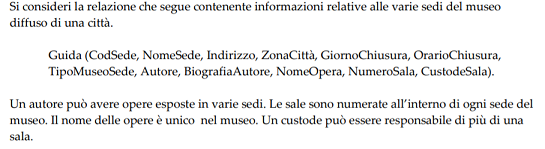
\includegraphics{images/222.PNG}
\end{center}
\begin{itemize}
	\item \textbf{Individuare la chiave e tutte le dipendenze funzionali non banali}:
	\begin{itemize}
		\item Osservazioni:
		\begin{itemize}
			\item La frase \emph{Un autore può avere opere esposte in varie sedi} esclude l'esistenza di una dipendenza funzionale dove la sede dipende dall'autore
			\item La frase \emph{Le sale sono numerate all'interno di ogni sede del museo} stabilisce che il numero sala non può essere da solo, sia nel lato sinistro che nel lato destro. Due sedi possono avere sale con le stesse numerazioni.
			\item La frase \emph{Il nome delle opere è unico nel museo} ci da la certezza che stiamo parlando di una certa opera realizzata da un certo autore.
			\item La frase \emph{Un custode può essere responsabile di più di una sala} indica che un custode si può occupare di più di una sala. Escludo quindi una dipendenza funzionale in cui il custode determina la sala.
		\end{itemize}
		\item Quindi individuiamo:
		\begin{itemize}
			\item Qua poniamo le informazioni riguardanti una sede, raggiungibili in modo univoco attraverso \emph{CodSede}
			\[CodSede \to NomeSede, Indirizzo, GiornoChiusura, OrarioChiusura, TipoMuseoSede\]
			\item La zona della città, pur essendo un dato relativo alla sede, non risulta direttamente dipendente dal codice della sede. La collocazione della sede in una certa zona della città si intuisce dall'indirizzo della sede. Segue
			\[Indirizzo \to ZonaCitta\]
			\item Gli attributi riguardanti le informazioni sull'autore sono \emph{Autore} e \emph{BiografiaAutore}. L'autore determina la biografia, segue
			\[Autore \to BiografiaAutore\]
			\item L'opera è realizzata da un certo autore ed è collocata in una certa sala. Abbiamo più sedi dove le numerazioni possono coincidere, segue
			\[NomeOpera \to CodSede, NumeroSala, Autore\]
			\item Ad ogni sala è associato in modo univoco un certo custode. Sapendo che le numerazioni possono coincidere in più sedi segue
			\[CodSede, NumeroSala \to CustodeSala\]
			\item La chiave, non indicata in anticipo, è \emph{NomeOpera}: questo è l'unico attributo che non compare nel lato destro delle varie dipendenze funzionali. La chiave è verificabile ricorrendo al calcolo della chiusura transitiva ${NomeOpera}^{+}$ rispetto all'insieme delle DF trovate prima.
		\end{itemize}
	\end{itemize}
	\item \textbf{Verificare se \emph{Guida} è in 3NF e, se non lo è, portarla in 3NF}:
	\begin{itemize}
		\item Risulta facilmente intuibile che non siamo in 3NF: data una qualunque dipendenza funzionale
		\[X \to Y\]
		$X$ non è mai superchiave e in $Y$ si individuano sempre attributi che non appartengono alla chiave candidata.
		\item Costruisco una relazione a partire da ogni singola DF introdotta prima. Otteniamo quanto segue
		\begin{center}
			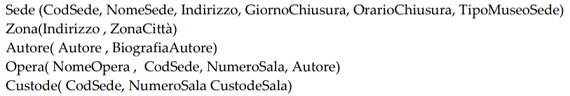
\includegraphics{images/226.PNG}
		\end{center}
		\item Adesso si ha la 3NF, poichè $X$ è sempre superchiave. 
		\item La chiave candidata, costituita da una solo attributo, non viene divisa dalla creazione delle varie relazioni. Segue che non è necessario creare un'ulteriore relazione contenente la chiave!
	\end{itemize}
\end{itemize}
\pagebreak

\section{Esercizio 2}
\begin{center}
	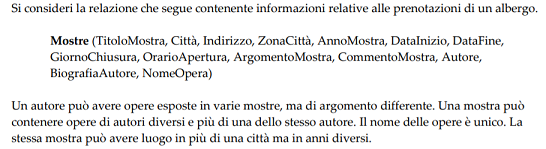
\includegraphics{images/223.PNG}
\end{center}
\begin{itemize}
	\item \textbf{Individuare la chiave e tutte le dipendenze funzionali non banali}:
	\begin{itemize}
		\item Osservazioni:
		\begin{itemize}
			\item La frase \emph{Un autore può avere opere esposte in varie mostre, ma di argomento differente} stabilisce che non possiamo stabilire una dipendenza del tipo $Autore \to TitoloMostra$.
			\item La frase \emph{Una mostra può contenere opere di autori diversi e più di una dello stesso autore} stabilisce che non possiamo avere DF del tipo $TitoloMostra \to Autore$.
			\item La frase \emph{Il nome delle opere è unico} stabilisce che globalmente ogni opera ha un nome diverso. Posso avere in mostre diverse la stessa opera ma non possono esistere due opere diverse aventi lo stesso nome.
			\item La frase \emph{La stessa mostra può avere luogo in più di una città ma in anni diversi} stabilisce che una mostra può tenersi in più città, ma che queste città non possono ospitare la mostra nello stesso anno.
		\end{itemize}
		\item Quindi individuiamo:
		\begin{itemize}
			\item Qua poniamo le informazioni riguardanti una mostra \underline{svolta in una certa città}, raggiungibili in modo univoco attraverso \emph{TitoloMostra} e \emph{AnnoMostra}. Ricordiamo che la mostra può avere luogo in più città, ma in anni diversi.
			\begin{align*}TitoloMostra, AnnoMostra \to\;& Citta, Indirizzo, DataInizio, DataFine, GiornoChiusura,\\&OrarioApertura\end{align*}
			\item La zona della città, pur essendo un dato relativo alla mostra non risulta direttamente dipendente da \emph{TitoloMostra} e \emph{AnnoMostra}. La collocazione della mostra in una certa zona della città si intuisce dall'indirizzo della mostra e dalla città. Segue
			\[Citta, Indirizzo \to ZonaCitta\]
			\item Gli attributi riguardanti le informazioni sull'autore sono \emph{Autore} e \emph{BiografiaAutore}. L'autore determina la biografia, segue
			\[Autore \to BiografiaAutore\]
			\item Gli attributi riguardanti le informazioni \underline{sul contenuto} della mostra sono \emph{TitoloMostra}, \emph{ArgomentoMostra} e \emph{CommentoMostra}. Gli ultimi due dipendono dal primo, quindi
			\[TitoloMostra \to ArgomentoMostra, CommentoMostra\]
			\item Il nome delle opere è unico globalmente, quindi sono certo che
			\[NomeOpera \to Autore\]
			\item La chiave, non indicata in anticipo, è \emph{TitoloMostra, AnnoMostra, NomeOpera}: questi attributi non compaiono nei lati destri delle varie dipendenze funzionali. La chiave è verificabile ricorrendo al calcolo della chiusura transitiva ${TitoloMostra, AnnoMostra, NomeOpera}^{+}$ rispetto all'insieme delle DF trovate prima.
		\end{itemize}
	\end{itemize}
	\item \textbf{Verificare se \emph{Mostre} è in 3NF e, se non lo è, portarla in 3NF}:
	\begin{itemize}
		\item Risulta facilmente intuibile che non siamo in 3NF: data una qualunque dipendenza funzionale
		\[X \to Y\]
		$X$ non è mai superchiave e in $Y$ si individuano sempre attributi che non appartengono alla chiave candidata.
		\item Costruisco una relazione a partire da ogni singola DF introdotta prima. Otteniamo quanto segue
		\begin{center}
			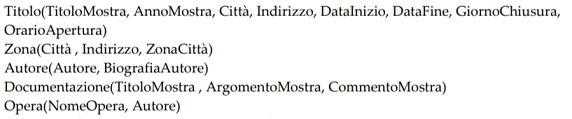
\includegraphics{images/227.PNG}
		\end{center}
		\item Non abbiamo ancora la 3NF poichè la chiave candidata non è presente nella sua interezza in nessuna delle chiavi delle varie relazioni. Segue la necessità di creare un'ulteriore relazione, la seguente
		\[Chiave(TitoloMostra,AnnoMostra,NomeOpera)\]
		Adesso siamo in 3NF!
	\end{itemize}
\end{itemize}